\scanpage{130}
\mspage{64}
the vertical \unsure{fibers|arrows} are morphisms
of extensions by kernels which are twisted $\mathbb Z^{d_0}$'s
-- in fact by the local systems
$T_{d_0}$, and its inverse image on $D^*_{d_0,-,d_r}$ --
we therefore \unsure{set|shall set}
\margin{at least if the $\unsure{\Pi_2|\pi_2}$ of $D_{d_0}^{\unsure{\circ|0}}$ and $D^*_{d_0,\unsure{-,|-}d_r}$ are zero...}
\[
\tag{2\unsure{1|6|0}0}
\left\{\begin{aligned}
T_{d_0,-,d_r}&=\text{inverse image }\unsure{\text{of}|\text{of the}}\text{ }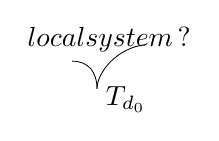
\begin{tikzpicture}[baseline=(t.base)]
\node[inner sep=0pt] (t) {$T_{d_0}$};
\node[anchor=south,inner sep=0pt] at ([xshift=-6pt,yshift=12pt]t.north) {$\text{local system}\,\unsure{\text{?}}$};
\draw[line width=.3pt] ([xshift=-12pt,yshift=9pt]t.north west) .. controls ([xshift=-6pt,yshift=9pt]t.north west) and ([xshift=-3pt,yshift=5pt]t.north west) .. ([xshift=-3pt,yshift=-1pt]t.north west);
\draw[line width=.3pt] ([yshift=15pt]t.north east) .. controls ([xshift=-3pt,yshift=14pt]t.north) and ([xshift=-3pt,yshift=5pt]t.north west) .. ([xshift=-3pt,yshift=-1pt]t.north west);
\end{tikzpicture}
\overset{\inserted{(\overset{\mathrm{locally}}{\simeq}\mathbb Z^{d_0})}}{
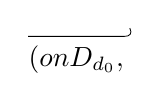
\begin{tikzpicture}[baseline=(s.base)]
\node[inner sep=0pt] (s) {$\text{ (on }D_{d_0},$};
\draw[line width=.3pt] ([yshift=3pt]s.north west)--([yshift=3pt]s.north east) .. controls ([xshift=2pt,yshift=3pt]s.north east) and ([xshift=3pt,yshift=4pt]s.north east) .. ([xshift=2pt,yshift=6pt]s.north east);
\end{tikzpicture}}\\
&\qquad\text{under }D_{d_0,-,d_r}\mathrel{\tikz[baseline=-.5ex,x=1em,y=1em]{\draw[line width=.45pt,line cap=round] (0,0)--(1.15,0)--(1.10,-.08);}}D_{d_0}\\
\deleted{T^*_{d_0,\unsure{-},d_r}=}
&\simeq\text{local system of the }\unsure{\Pi_1|\pi_1}\text{ (or of the }H_1\text{)}\\
&\qquad\text{of the fibres of }P_{d_0-d_r}\text{ over }D_{d_0-d_r}\\
T^*_{d_0-d_r}&=T_{d_0-d_r}\mid D^*_{d_0,-,d_r},
\end{aligned}\right.
\]
so that $\widetilde\Pi_{d_0,-,d_r}$ is an extension of
$\Pi_{d_0,-,d_r}$ by $T^*_{d_0,-d_r}$.
\margin{at least if $\unsure{\Pi_2|\pi_2}(D^*_{d_0,-d_r})=0\ldots$}

We shall of course set
\[
\deleted{\unsure{\widetilde\Pi_{*\Delta_r}|\Pi_{\Delta_r}}=\coprod\Pi_{d_0,-,d_r}}
\]
\[
\tag{211}
\left\{\begin{aligned}
\unsure{G_{\Delta_r}|B_{\Delta_r}}&=
\coprod_{\substack{\deleted{\unsure{d_r\geq-\geq d_0}}\\(d_0,\mathord{-\, -},d_r)\in\mathbb N^{r+1}\\d_0\geq d_1\,{\cdot\, -}\,\geq d_r}}
\unsure{B_{d_0,-d_r}|G_{d_0,-d_r}}\qquad\text{group over }D_{\Delta_r}\\
P_{\Delta_r}&=\coprod P_{d_0,-,d_r}\qquad\text{torsor under }G_{\Delta_r}\\
T_{\Delta_r}&=\coprod T_{d_0,-,d_r}\qquad\text{local system of the}\\
&\hspace{4cm}\unsure{\Pi_1|\pi_1}\text{, }\unsure{\text{or}}\ H_1\text{, of}\\
&\hspace{4cm}G_{\Delta_r}\ \mathrel{\tikz[baseline=-.5ex,x=1em,y=1em]{\draw[line width=.45pt,line cap=round] (0,.07)--(.15,.14); \draw[line width=.45pt,line cap=round] (.27,0)--(1.05,0);}}\ P_{\Delta_r},\ \mathrel{\tikz[baseline=-.5ex,x=1em,y=1em]{\draw[line width=.45pt,line cap=round] (0,.08)--(.14,.10); \draw[line width=.45pt,line cap=round] (.26,0)--(1.02,0);}}\\
G^*_{\Delta_r},\ P^*_{\Delta_r},\ T^*_{\Delta_r}&\qquad\unsure{\text{say}|\text{will say}|\text{dés}}\\
&\qquad\text{the restrictions to }D^*_{\Delta_r}
\end{aligned}\right.
\]
\margin{129}
